\documentclass[11pt,oneside]{article}
\usepackage{fullpage}

%%% Load some useful packages:
\usepackage{graphicx}
\graphicspath{{figures/}}
\usepackage{subfigure}
\usepackage{bbm}
\usepackage{tabularx}
\usepackage{setspace}
\onehalfspacing
%% Package to linebreak URLs in a sane manner.
\usepackage{url}

\usepackage{todonotes}
\usepackage{amsmath,amsfonts}
\numberwithin{equation}{subsection}
%% Define a new 'smallurl' style for the package that will use a smaller font.
\makeatletter
\def\url@smallurlstyle{%
  \@ifundefined{selectfont}{\def\UrlFont{\sf}}{\def\UrlFont{\small\ttfamily}}}
\makeatother
%% Now actually use the newly defined style.
\urlstyle{smallurl}

%% Define 'tinyurl' style for even smaller URLs (such as in tables)
\makeatletter
\def\url@tinyurlstyle{%
  \@ifundefined{selectfont}{\def\UrlFont{\sf}}{\def\UrlFont{\scriptsize\ttfamily}}}
\makeatother

%% Provides additional functionality for tabular environments
\usepackage{array}

%% Puts space after macros, unless followed by punctuation
\usepackage{xspace}

%% Make margins less ridiculous
\usepackage{fullpage}

%% Allows insertion of fixme notes for future work
\usepackage[footnote, nomargin]{fixme}

%% Make URLs clickable
\usepackage[colorlinks, bookmarks=true]{hyperref}

\begin{document}
\title{Contribution chapter abstract for Ph.D. dissertation: \\
       \textsc{Software Trajectory Analysis:} \\
       \textsc{An empirically based method for automated software process discovery} \\
       \author{Pavel Senin \\
               Collaborative Software Development Laboratory \\
               Department of Information and Computer Sciences \\
               University of Hawaii \\[0.3cm]
               \texttt{senin@hawaii.edu} \\[0.3cm]
               CSDL Technical Report 09-13 \\
               \url{http://csdl.ics.hawaii.edu/techreports/09-13/09-13.pdf}
       }
       \date{February 2013}
}
\maketitle

\clearpage


\section{Introduction}
Software engineering is a unique area of engineering field, blessed with having no cost 
associated with materials and fabrication, which dominate other areas of engineering. 
However, ironically, software engineering is suffering from the costs and challenges
associated with continuous re-design of the software design (development ) processes, 
which is rarely seen at all in any other engineering areas. 

In order to efficiently deal with this issue, many universal design processes - known as 
software development methodologies - were proposed up to date. 
For example, the Waterfall Model process proposes a sequential pattern in which developers 
first create a Requirements document, then create a Design, then create an Implementation, 
and finally develop Tests. 
In contrast, the Test Driven Development process proposes an iterative pattern,
in which the developer  must first write a test case, then write the code to implement 
that test case, then refactor  the system for maximum clarity and minimal code duplication.

One problem with the  traditional top-down approach to software process design is that it 
requires the developer or manager to ``invent'' the process in the first place. Whether
through noticing of recurrent development patterns, or through a decomposition of a larger 
problem, invention is a difficult task \cite{citeulike:5043104}. 
Another problem, is that process inventors, limited in their scope, 
always assume an idealized versions of real processes and tend to produce ``paper lions'' - 
process models which are likely to be disruptive and  unacceptable for end users, at least 
in their proposed form \cite{citeulike:9758924}. In addition to these facts, the full study 
cycle from a process proposal, through its evaluation, to its full understanding is 
usually measured by decades \cite{citeulike:113403}.

In my research, I attempt to contribute to an alternative - the bottom-up - approach to software
process design. The idea ``at large'', is that through the observation of the performed 
by developers processes it is possible to notice recurrent behaviors, which could be
further generalized and associated with building blocks of a larger software development process
model. The idea of inferring a process model through observing and studying performed processes is
not new and was around for decades \cite{citeulike:328044}. While cutting down on the
evaluation time when compared to ``process invention'', there is a number of problems also - there
are privacy issues, overall cost of the observations, and its overall validity. The key issues
behind these is the vital necessity of on-line observation and interpretation, interviewing and
coding.

In my work, I am addressing these core issues through leveraging of knowledge discovery techniques
applied to software artifact trails. For this, I have designed a process analysis 
methodology built upon a novel technique for knowledge discovery from temporal data. 
These two pieces - the novel, generic technique of knowledge discovery from temporal data,
and the exploratory study of its application to software development artifacts trails 
are the main contributions of my thesis.

\subsection{Mining of software process artifacts}
In my PhD thesis proposal, outlining the plan of work, I have mentioned that ``...many temporal
knowledge discovery and data mining methods developed in the last decade can be applied to the
software process domain...'', which turned out to be a bit of overstatement. It is only during 
their evaluation on the real data, I have realised that most of them produce insensible results,
especially those, which are based on the sequential events analysis, or assume a periodicity.

While these is a ``shot from the hip'' (a speculative statement, which requires additional
research to be done), from my own experience, the failure of common sequential or associative 
pattern mining techniques can be directly contributed to the granularity of my data. The numerous
software process artifacts, that I have collected from public software repositories, just do not
reflect all those essential atomic events such as coding, compiling, building, and testing.
Moreover, events which are possible to recognize, such as change, are misplaced in time by the
commit process. 

The failure of time series analysis techniques based on the periodicity and consistent ordering
happens due to the intristic aperiodicity and disordered nature of developers behaviors.
That is - software is coded by humans and is a human-driven process. 
And this is exactly where the problem lies - in the way teams and individuals
perform relevant daily activities in order to reach the goal - deliver the software.
Humans do not work on a pre-defined schedule - we have all sorts of distractions 
during development time - phone calls, meetings, co-workers popping in, emails, etc.
Developers could take a sick leave, or just take a day off to go to the football game,
or just get stuck solving a programming problem, or pause in order to help solving one.
Also, without any time and space constraints in the contemporary ``connected'' world,
developers could start coding literally at the middle of the night or during long 
commute on train or airplane. Thus, we must assume here, that the
data I am working with in this thesis is not only large, but noisy, and aperiodic.

Moreover, it is important to understand, that this data is essentially a product of two
components. First compoent is a behavioral one - the human-driven, non-recurrent, aperiodic,
creative process of coding, while second component is the technology and methodology in use.
\todo[inline]{connect better}.
While latter probably provides a potentially well-measurable, marginal effect, it is another 
source of noise in the data.

This assumptions invalidate most of temporal data mining techniques. In particular,
any of techniques leveraging the finding a periodicity, such as Fourier transform-based 
ones, or Wavelets, will most likely fail. Further, any time-series technique based 
on the convenient, non-elastic, metrics - such as Euclidean - probably would fail too.

Apparently, there are very few tools left as shown at the
Figure \ref{fig:timeseries-representations}. \todo{elaborate and connect tools and representations}

\begin{figure}[tbp]
   \centering
   \includegraphics[height=40mm]{representations.eps}
   \caption{A hierarchy of all the various time series representations in the literature from
       \cite{citeulike:2821475}. The leaf nodes refer to the actual representation, and the internal
            nodes refer to the classification of the approach.}
   \label{fig:timeseries-representations}
\end{figure}



 Temporal data are 
Many data mining tasks are based on datasets containing sequential characteristics, such
as web search queries, medical monitoring data, motion capture records, and astronomical
observations. In these and many other applications, a time series is a concise yet expressive
representation. A wealth of current data mining research on time series is focused on providing exact solutions in such small datasets. However, advances in storage techniques and
the increasing ubiquity of distributed systems make realistic time series datasets orders of
magnitude larger than the size that most of those solutions can handle due to computational
resource limitations. On the other hand, proposed approximate solutions such as dimensionality reduction and sampling suffer from two drawbacks: they do not adapt to available
computational resources and they often require complicated parameter tuning to produce high
quality results.

aTo alleviate This phenomena still poorly understood and thus, there is nhas driven software process research 
This e reason for this continuous d

Its been \cite{citeulike:11061107}
feature of software engineering, recognition includes two fundamental tasks: description and classification. Given
a process, a recognition system first generates a description of it (i.e., reconstructs the process in
full or partially) and then classifies the process based on that description (i.e., the recognition).

Two general approaches for implementing pattern recognition systems, statistical and structural, employ differ-
ent techniques for description and classification. Statistical approaches to pattern recognition use
decision-theoretic concepts to discriminate among objects belonging to different groups based upon
their quantitative features. Structural approaches to pattern recognition use syntactic grammars
to discriminate among objects belonging to different groups based upon the arrangement of their
morphological (i.e., shape-based or structural) features. Hybrid approaches to pattern recognition
combine aspects of both statistical and structural pattern recognition.

Many engineering, scientific, and production fields (such as movie-making or advertisement) have explicit 
and formalized design processes which are well studied to at least some degree. In contrast, in software 
development we are treating the process of design itself as a thing to be designed and, potentially, 
re-designed along the way. While there are ``best practices'', they prone to fail and it is commonplace
to alter these through combination or a systematic change.



Software artifacts are abundant and thought to carry a significant amount of information about performed 
processes.

However, the vast majority of artifacts are concerned about the software itself and largely associated 
with a specific development methodology. Examples of such artifacts are design documents, use cases, class 
diagrams and requirements, user manuals, etc. The payload of this artifacts aids in understanding of 
a function, architecture, and the design of software, while carrying a very little information about the 
applied effort and underlying behaviors. Due to this fact, I put such artifacts outside of this thesis
immediate attention.

What is studied in this work, is the informational content of software development process byproducts 
which accompany software change. It is long known that change Change not only provides an evidence about performed activities, and, potentially, 
carry an informational load about
recurrent behaviors. Such artifacts span in time, as behaviors do, and usually reflect both: the applied 
effort (process), and the evolution of the software itself. 
Examples of such artifacts are source code changes, bug reports, and developers discussions.

Note, however, that developers do not intentionally create these artifacts to enable research, or to keep 
things in some order - mainly, these artifacts are the pure byproduct helping to the development of a 
software project. Thus, we must assume here, that this data is inconsistent, that any kind of annotations 
used by developers might be erroneous, and the amount of disclosed information could simply be not enough
to determine the actual generative behavior - which ultimately leads to uncertainty of any claims about
process correctness, ``productivity'', or any other performance-related metrics. 

The focus of my work is to explore the informational content of software process artifacts designing 
a toolkit capable to handle the discovery of recurrent behaviors automatically. Ideally, such a toolkit 
must have following properties:
\begin{itemize}
 \item it must be Effective: the reported findings, with respect to behaviors reconstruction, must agree 
 with human intuition.
 \item it should be Scalable: currently software process artifact trails for a single project could easily 
       grow beyond dozens of gigabytes, thus, the computation technique should ideally be able to utilize 
       parallelization and be capable to pre-compute intermediate results alleviating the overall space-time 
       complexity to enable an online (fast turn-around) interactive mining.
 \item Efficient: the set of reported findings should not exceed a certain threshold simly becoming an 
        overwhelming stream of spurious facts.
\end{itemize}


\section{Methodology}
Given multiple trails of software process artifacts, how to find recurrent behaviors? In this chapter, 
I will describe the design and an implementation of research methodology employed in Software Trajectory 
Analysis. In short, the implemented approach enables aggregation, indexing and mining of software 
artifact trails allowing the discovery of recurrent behaviors. 

\section{Temporal attributes of software process artifacts}
The close examination and analysis of temporal dynamics of artifact-generating events laying the foundation 
of STA methodology. The extraction of software process-related metrics, their temporal partitioning and the
ability of finding the relevant information is the 



%%% Input file for bibliography
\bibliography{seninp}
%% Use this for an alphabetically organized bibliography
\bibliographystyle{plain}
%% Use this for a reference order organized bibliography
%\bibliographystyle{unsrt}
%% Try using this BibTeX style that hopefully will print annotations in
%% the bibliography. This will allow me to make notes on papers in the
%% BibTeX file and have them readable in the references section until
%% I turn them into a conceptual literature review 
%\bibliographystyle{annotation}

\end{document}
